\documentclass[sigconf,authorversion,nonacm]{acmart}
\bibliographystyle{ACM-Reference-Format}
\usepackage{hyperref}
\usepackage{alltt}

%TODO: disable folios
\settopmatter{printfolios=true}

\definecolor{ForestGreen}{RGB}{34,139,34}

%\widowpenalties 4 0 9000 10000 10000

%%%%%Prof Zhou's Rant on Citations, Punctuation, and Quotes %%%%%%
%%%
%%% Yes - ...of seventy-two''~\cite{42}.
%%% Yes - ...of seventy-two.''\footnote{42}
%%%
%%% NO! - ...of seventy-two.''~\cite{42}.
%%%
%%% https://advice.writing.utoronto.ca/wp-content/uploads/sites/2/quotations.pdf
%%%
%%%%%%%%%%%%%%%%%%%%%%%%%%%%%%%%%%%%%%%%%%%%%%%%%%%%%%%%%%%%%%%%%%

% 8-10 pagecount.

\begin{document}
\title[Visualizing CAD changes with Boolean Differences]
{Visualizing CAD changes with Boolean Differences\\
	\normalsize{Group 25 Final Report}}
%I'd like to remove the 'group 25 report' from the title, not really sure where to put it though .

\author{Amos Hebb}
\affiliation{\institution{University of Toronto}}
\email{a.hebb@mail.utoronto.ca}
\author{Yilong Wang}
\affiliation{\institution{University of Toronto}}
\email{yilongece.wang@mail.utoronto.ca}
\author{Zhenyue Yu}
\affiliation{\institution{University of Toronto}}
\email{zhenyue.yu@mail.utoronto.ca}

\makeatletter
\def\@ACM@checkaffil{% Only warnings <<<<<<<<<<<<<<<<
	\if@ACM@instpresent\else
		\ClassWarningNoLine{\@classname}{No institution present for an affiliation}%
	\fi
	\if@ACM@citypresent\else
		\ClassWarningNoLine{\@classname}{No city present for an affiliation}%
	\fi
	\if@ACM@countrypresent\else
		\ClassWarningNoLine{\@classname}{No country present for an affiliation}%
	\fi
}
\makeatother

\maketitle

\section{Introduction}

TODO:This section will include the background of our project and introduce computer-aided design (CAD), OpenSCAD, GIT and Boolean differences. In this section, we will also outline our research question and discuss the motivation behind its development.

\subsection{CAD}

TODO:Definition and significance of CAD in complex product design and development. Description of challenges associated with distributed CAD practice.

\subsection{OpenSCAD}

\subsection{\texttt{.stl} files}

The \texttt{.stl} file format is a representation of the surface geometry of a three-dimensional object common in both CAD and 3D art.
These files are among the \textit{dumb solid} types described in \cite{cheng2023age}, a neutral file format interoperable between most CAD and 3D art platforms, but missing critical information for CAD practitioners.
\texttt{.stl} files have no way to represent curves, holes, orientation, or distinguish multiple parts in an assembly.
Providing measurements is optional in \texttt{.stl} files. CAD programs usually store this optional information about units.
We hope this tool can be used with any CAD software.
Most CAD programs support exporting models to \texttt{.stl} files and our visualization only relies on surface geometry, making \texttt{.stl} files appealing for producing quick summaries.

\subsection{Git}

Git is a version control system designed by the Linux kernel team to support many coders making changes to text files in a distributed and collaborative way.
Git has become one of the most widely used version control systems and is particularly popular in open-source development projects which face similar challenges to the Linux kernel team.
It has many powerful utilities for manipulating text files.
While Git can handle binary files, the utilities that make it so useful for the collaborative editing of text files do not exist for the complex binary files used in 3D CAD.

\texttt{git diff} is a utility that allows a user to see changes.
These changes are represented by insertions and deletions.
For example, running \texttt{git diff} on a branch where a punctuation mark is added to a hello world program will show unchanged lines in black, insertions in green, and deletions in red.

\begin{alltt}
	fn main ()\{
	\textcolor{red}{   - println!("Hello World");}
	\textcolor{ForestGreen}{   + println!("Hello World!");}
	\}
\end{alltt}

Integrated development environments, git hosts, and other command line tools present git diff with different formatting, layout, and truncation of unchanged code.
There is one thing that unifies every visualization of \texttt{git diff}, the red deletions and green insertions visual.
This red and green visual is ubiquitous in code tools, it is the default presentation of a branch, merge, history, and pull request on every major git platform and every integrated development environment with git support.
These clear visual representations of the differences between different versions of a file make it easy for developers to see what has changed and where.

\texttt{git cherry-pick} is a less common git command.
A developer checks out a target branch and then runs the \texttt{git cherry-pick} with a commit hash to apply a specific commit to the target branch.

It is typically used when there are changes in a \emph{feature} branch that one wishes to apply to the \emph{target} branch.
Instead of merging the entire \emph{feature} branch into \emph{target}, which would bring in all the changes in \emph{feature}, \texttt{git cherry-pick} is used to apply only the specific commits desired.
To do this, a developer would first identify the commits in the \emph{feature} branch that apply the changes they wish to apply.
The developer would \texttt{git checkout} the \emph{target} branch.
The developer then uses \texttt{git cherry-pick} command to apply those commits to the \emph{target} branch.
This creates a new commit in \emph{target} that contains only the changes from the selected commit in \emph{feature}.

A concrete example grounded in 3D CAD.
A company produces a teapot which is modeled in 3D CAD file saved as `main'.
Three changes are made to this initial file.
First, the spout is shortened.
Second, the handle is made square.
Third, the knob on top is made bigger.
The resulting prototype file is saved as `v2', and has a short spout, square handle, and large knob.
After prototyping, the company wishes to keep the short spout and large knob, but keep the original handle.
Only the two desired changes from `v2' are applied to `main', resulting in `main2' with the desired changes.

\subsection{Boolean Differences}

TODO:Explanation of Boolean differences visualization techniques and how visualizations of Boolean differences can be an alternative to current methods for summarizing changes between CAD file versions.

\section{Literature Review}

TODO:The motivating paper for this project is \citet{cheng2023age}. The author of this paper also guided us to existing tools, such as \texttt{onshape.com}, which implement similar visualizations.

\subsection{\texttt{onshape.com}}

An existing tool, \texttt{onshape.com}, was evaluated as part of this review.
We were able to create an account and get access to Daniel Riley's Sailboat
%https://cad.onshape.com/documents/a8a8056c3b88f0daf9611dcb/w/221f8e757824bdfe5ba7440b/e/ee5cdb3266c7d6966d32f749
which is a public model which shows a rich combination of \texttt{onshape.com}'s capabilities, in particular, once signed in, the `Versions and History' tab.
This shows a branching visual, with symbols for versions, releases, and the current workspace.
This is initially collapsed, with only versions showing, but expanding a version shows each of the modifications applied.
These modifications are clearly automatically generated, as they are far more granular than would typically be checked into version control manually.
For example, many trivial `Hide', `Show', and long chains of `Drag, Drag, Drag, Drag' and `Move, Move, Move, Move' where the CAD designer seems to be making minor intermediate adjustments.
By default, no `diff' like view is shown.
Instead, the entire document re-loads when clicking on any change.
Right-clicking does reveal a `Compare' option, instead of just `View'.
Many changes throw an error, for example, comparing Main `Show:Keel Mold - Daniel Riley - 1:01 PM Mar 8 2023' to one change before it, the `Move:Rollback bar - Daniel Riley - 12:18 PM Mar 8 2023' removes the render from the screen and shows the error message ``NOT COMPARABLE: Comparing Assemblies is not yet supported.''
Selecting individual components reveals \texttt{onshape.com}'s comparison interface.
The assembly is scattered into an unwieldy exploded view where parts overlap.
Instead of rendering boolean differences, \texttt{onshape.com} renders a before and after visual, and allows a user to scroll a slider left to right while moving the entire exploded state around.
Subtractions are highlighted in red, while new volumes are rendered in blue.
Figure \ref{fig:onshapescreenshot} shows a screenshot with the slider roughly 2/3 toward the new component, showing a partially transparent blue volume, and orange-red holes being cut.

\begin{figure}[t]
	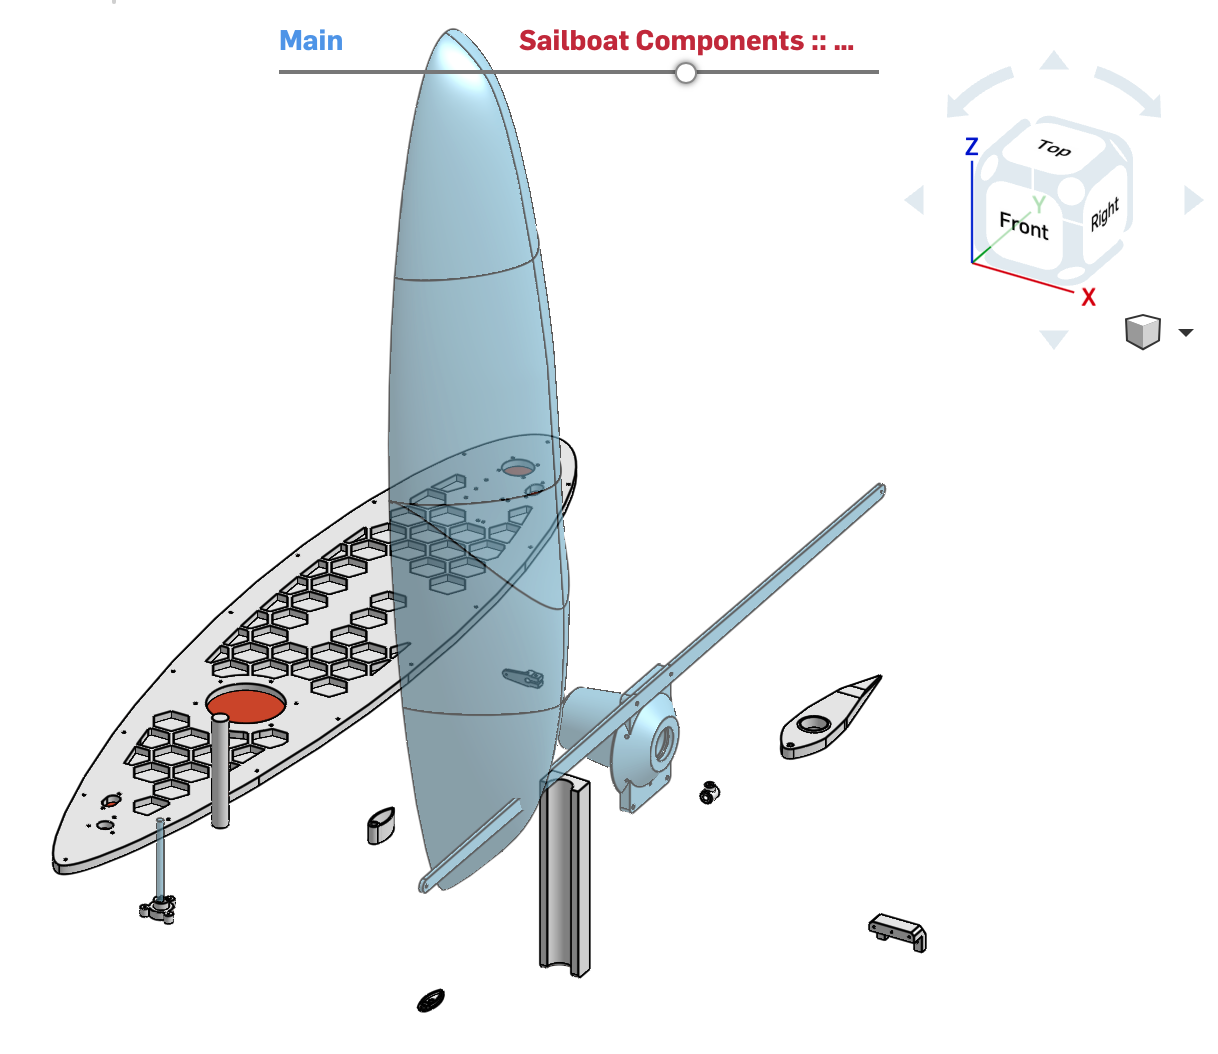
\includegraphics[width=\linewidth]{onshapescreenshot.png}
	\caption{Example of \texttt{onshape.com} compare visual}
	\label{fig:onshapescreenshot}
\end{figure}

\subsection{Previous Work}

TODO:Summarize the findings from \citet{cheng2023age}  that explores distributed teams, version control, and summarization of changes between CAD file versions.
TODO:We will provide a concise overview of a chapter from \citet{Frazelle_2021} on version control to justify the use of \texttt{GIT}-like semantics.

\subsection{Existing CAD Version Control}

TODO:We will provide a summary of the concepts we will adopt from GitHub's \citet{github_blog_2013} and the implementation of the change detection solution discussed in \citet{3drepo_blog}.
TODO:Additionally, we will outline GrabCAD's Cosmo Quiz\cite{revisions_2014}, an initiative aimed at codifying current best practices in CAD work.
TODO:Furthermore, we will condense the information on change management and version control mechanisms from \citet{Bricogne_Rivest_Troussier_Eynard_2012}, while also highlighting the identified opportunities for improvement.

\section{Methodology}

TODO:Subsections will outline details of both our proposed experiments, including refinements made as a result of the feedback described in Appendix A.

\subsection{Timed Cherry-Picking Experiment}

\subsubsection{Participants}

The participants are randomly assigned to one of two groups: the experimental group and the control group.
We expect that individual participants may have different levels of experience with each of CAD tools, version control tools, and 3D Art tools.
Recruiting participants with experience in all three will be difficult, so instead we will design our experiment assuming no prior knowledge of any of the above.
We rely on simple random assignment to keep familiarity with the above tools similar between the two groups.
Participants will be informed of the purpose of the experiment and their rights as participants.
Participants who wish to complete this experiment virtually will require a connection to the internet and a web browser with WebGL support.
Participants may also complete this experiment in person using a computer provided by experimenters.
Only completion times and accuracy scores will be recorded with no way to link times back to individual participants.
Participants will be informed that data will be openly available in a public repository that does not issue DOIs.
Participants may withdraw from the experiment at any time and incomplete results will be discarded.

\subsubsection{Task}

The participants will be tasked with reversing a certain part of an object back to a previous version while keeping the rest of the object the same as the final version.

As we assume participants are not familiar with version control, CAD, or 3D art tools, we will not use any existing tools in the experiment to reduce the effect of prior exposure to any of these tools.
Version control tools have specific commands that are not intuitive, and both CAD and 3D art tools have very complex interfaces that could distract participants.
We instead produce a stripped-down interface which only allows participants to view files, and mark files to be included or excluded.

%Attached are screenshots from both the control and experimental group. 
%Figure \ref{fig:controlscreenshot} shows a screenshot of the interface that will be shown to the control group.
The interface has two frames which will render a webGL view \texttt{.stl} renderings of our revisions.
Participants do not need to know file formats, and instead will just refer to changes as an enumerated list of `Original, Change 1, Change 2, Change 3 refer to changes as an enumerated list `Original, Change 1, Change 2, etc.'.
Below each of these frames is a drop-down menu allowing participants to select any of the change files.
The task goal is displayed below these frames.
Below the task goal is a list of changes, along with a radio button group with labels `Include' and `Exclude', which by default will not be selected.
To complete a task, participants must select one of `Include' or `Exclude' for every change, and then press the `Submit' button.
%Figure \ref{fig:experimentscreenshot} shows a screenshot of the interface that will be shown to the experiment group.
The \textbf{experimental group} will have a 3rd frame.
This 3rd frame will render the red and green \emph{diff} view produced by performing boolean operations on the two selected files.


\subsubsection{Procedure}

Before the experiment begins, participants may complete a practice task with assistance from the experimenters as many times as they desire.
Once participants have indicated that they understand the task, experimenters will leave participants to complete the experiment on their own.

Only a `Begin' button will be shown.
Once clicked, a timestamp is logged, and the first task will be presented to the participant.
Once a participant has selected either `Include' or `Exclude' for each of the changes, the `Submit' button will be enabled.
Once a participant clicks the `Submit' button, a second timestamp is logged, along with the `Include' or `Exclude' status of every change.
The task is now over, and the `Begin' button will be shown for the next task.
Once a participant has completed 5 tasks, a `Thanks for participating' screen will be shown.

\subsubsection{Evaluation}

Accuracy will be measured by counting the number of correctly marked changes a participant has submitted to a reference solution.
Every task will have a canonical solution, with a certain set of commits labelled as either `include' or `exclude'.
We will compare this canonical solution to the solution produced by each participant and count the number of correctly labeled changes.
The fraction of correct labels will be our accuracy count, meaning that accuracy will be from 0-1 where 1 is perfect.

Time will be measured in seconds from when participants click the begin button until when they click the submit button.

\subsubsection{Data Analysis}

The first step in analyzing the data is to collect descriptive statistics for both accuracy and time.
These descriptive statistics will be used to confirm our assumptions about the distributions of both of these data.
We will also clean these data to remove any faulty submissions (time is impossibly fast, marked all files `Include', etc.).
Removed rows will be marked `True' in the column \texttt{removed\_from\_analysis} for the public dataset.

We expect times to be normally distributed about the task mean time for each task.
A T-Test will reveal if there is a difference in completion time for the same task between the two groups.
This test will allow us to accept or reject the following hypotheses.

$H_{0}$: Access to the boolean difference view has no impact on the completion time of cherry-picking changes in 3D files.

$H_{Time}$: Access to the boolean difference view reduces mean completion time of cherry-picking changes in 3D files.

As the tasks are fairly obvious, we expect accuracy will follow some long tail distribution with most participants making no mistakes, some making one or two, and rare unusually poor performing participants making many.
Applying statistics that are based on variance and standard deviation to accuracy scores will be impacted by single large outliers.
Instead, we will fit a Poisson distribution to the accuracy scores of each group treating each mistake as a discrete event, and then compare the rate at which mistakes are made between the two groups.
A C-Test~\cite{przyborowski1940homogeneity} is well suited for 0 included Poisson distributions to see if the rate of errors has been changed by the introduction of the Boolean difference view.
This test will allow us to accept or reject the following hypotheses.

$H_{0}$: Access to the boolean difference view has no impact on the accuracy of cherry-picking changes in 3D files.

$H_{Accuracy}$: Access to the boolean difference view reduces the rate of mistakes when cherry-picking changes in 3D files.

A reduction in time and mistakes will indicate that the boolean difference view helps summarize differences, as participants were able to more quickly and more accurately understand changes that had been made in 3D files when they had access to these visualizations.

\subsection{Summarization Experiment}
\subsubsection{Participants and Recruitment}
For the summarization experiment, we plan to recruit participants using purposive sampling. Our target population will consist of individuals with experience in CAD design, as indicated by the inclusion of ``CAD,'' ``CAD Design,''
or similar tags in the Skills section of their LinkedIn profiles. Potential participants will be contacted through LinkedIn messages. 

In our initial communication, we will provide an overview of the experiment's purpose and outline the main experimental procedures. 
This will help ensure that prospective participants have a clear understanding of what is involved before deciding to participate. As an incentive for their time and effort, those who complete the experiment will receive a \$25 gift card as compensation.

A table will be presented to summarize the demographic information of the participants, including their years of experience with CAD and related information such as whether they use CAD in their daily work.

\subsubsection{Experimental and Control Groups}

The study will use a randomized controlled design, in which participants will be assigned to either the experimental or control group by random assignment. This approach aims to eliminate confounding factors such as prior experience with 3D CAD Design or Git Diff. Assigning participants based on their experience level may introduce systematic error and relying on self-reported experience may not ensure a fair assignment. Therefore, the groups will be assigned by total random assignment.

Both groups will have access to the \texttt{.stl} file and the visualization of 3D objects. The experimental group will also have access to the visualization of Boolean differences. This approach will allow for a comparison between the two groups in terms of their ability to work with the Boolean difference visualization.
\subsubsection{Experimental Procedures}
This summarization experiment employs semi-structured interviews to explore the impact of Boolean difference visualizations on participants' ability to identify and describe changes between two 3D CAD objects.
The experiment consists of three distinct stages: preparation, inspection, and summarization, each designed to ensure a smooth and effective process. We anticipate the whole experiment will take 60 to 90 minutes to complete.

During the preparation stage, researchers take care to address participants' rights and confidentiality. They emphasize the voluntary nature of participation and confirm that participants understand the experiment's purpose and methodology.
To facilitate a successful experience, researchers provide a comprehensive walkthrough of the visualization platform's operation techniques. This includes demonstrating how to switch between \texttt{.stl} files, 3D object visualizations, and Boolean difference visualizations, when applicable.
Participants are given ample time to familiarize themselves with the platform and its features, ensuring they feel comfortable and confident before the experiment begins.

In the inspection stage, participants carefully examine the two CAD objects presented to them. Researchers adopt the role of non-participant observers, maintaining a neutral presence and refraining from answering any questions related to the objects, their differences, or the locations of changes.
The only exception to this rule occurs when a participant encounters a technical issue with the visualization platform.
In such cases, researchers step in to resolve the problem and ensure the participant can continue their inspection without further difficulties.

Once participants feel ready to proceed, they provide a summary of the changes they have identified between the CAD objects. Researchers carefully record their responses for future analysis.
Throughout this stage, participants are allowed to pause, return to the visualization platform for additional inspection, and resume their summary as needed. In cases where a participant's answer is too vague,
researchers may gently prompt them to refine their responses and include more specific details, all while avoiding the introduction of any hints or suggestions.

This experiment distinguishes itself by offering the experimental group access to visualizations of Boolean differences between the two objects, in addition to the standard \texttt{.stl} files and 3D object visualizations.
After completing the experiment, researchers ask members of the experimental group to provide feedback on how the Boolean difference visualizations impacted their summarization process.
By gathering these insights, researchers aim to better understand the potential benefits and drawbacks of this visualization technique.
These additional responses are also recorded and analyzed alongside the main summaries, contributing to a comprehensive understanding of the experiment's outcomes.

\subsubsection{Analysis}
The primary analysis methods for this study will be open coding and axial coding, which are essential components of qualitative data analysis. These methods will help researchers gain deeper insights into the participants' responses and identify potential patterns that emerge from the data.

Before initiating the coding process, researchers will convert the recorded responses into detailed transcripts. By reviewing these transcripts, they will familiarize themselves with the data and gain a foundational understanding of the participants' perspectives.

During the open coding phase, researchers will examine and label segments of the interviews. This process involves two researchers working independently to label the responses, after which they will compare and discuss their respective labeling results. 
This collaborative approach helps ensure the coding process is thorough and reduces potential bias or oversight.

If a segment is labeled by only one researcher, both researchers will carefully review it together and decide whether labeling is necessary. In cases where the same segment has been assigned different labels by the two researchers, 
they will first evaluate if the labels have the same underlying meaning. If so, they will agree on a single label to be used consistently throughout the coding process. 
If not, they will attempt to resolve their differences through discussion. Should a consensus remain elusive, a third researcher will be consulted to provide an impartial perspective and arbitrate the disagreement.

Once the open coding process is complete, researchers will transition to axial coding. This phase involves analyzing the relationships between the various codes and organizing them into cohesive subcategories and categories using a coding paradigm. 
Axial coding helps researchers refine their understanding of the data, discover connections, and identify overarching themes that may emerge from the participants' responses.

Specifically, the additional question and response regarding the impact of Boolean difference visualizations will be coded and triangulated with the coding results of the change summarizations. 
Through triangulation, researchers aim to identify patterns or themes consistent across both sets of responses. By analyzing and interpreting these patterns or themes, we hope to better understand the influence of Boolean difference visualizations on individuals' ability to interpret and summarize changes between CAD objects. 
This approach will provide valuable insights into the potential benefits and drawbacks of using Boolean difference visualizations in the context of CAD design analysis.

It is important to note that specific codes will be developed after the summary experiment is conducted. Based on the hypothesis, the researchers anticipate that the experimental group, 
which has access to the Boolean difference visualizations, will describe changes more intuitively. This might result in phrases such as ``the knob is larger in object A than in object B.'' 
In contrast, the control group, relying primarily on the \texttt{.stl files}, might describe changes using specific measurements, such as ``the radius of this knob is $2$ centimeters larger than before'' 
By employing open coding and axial coding techniques, the researchers aim to identify these and other potential patterns within the data, ultimately enhancing their understanding of the experiment's outcomes and the impact of different visualization methods on participants' summarization processes.

%TODO:We will provide further details on the experiment, highlighting the specific open-ended questions that will be employed during the interviews in conjunction with this study.

\section{Dataset}

TODO:The subsections will cover our carefully curated collection of OpenSCAD files with revisions, as well as their organization. Additionally, we will provide pre-compiled differences visualizations saved in \texttt{.stl} format for review by future researchers. These files will be sourced from the Git commit history of an open-source OpenSCAD project hosted on \texttt{github.com}, and from an open-source project on \texttt{onshape.com} with a complete modification history.
TODO:We will also include figures that demonstrate a before, after, addition, and subtraction example for a single, straightforward object.

\section{Results}

TODO:In this section, we will present and discuss the results we expect to get from each experiment.

\subsection{Timed Cherry-Picking Experiment}

TODO:We anticipate observing a difference in both the time taken to complete the task and the accuracy of responses between the experimental group and the control group. If Boolean difference visualizations aid in understanding the changes, we expect the experimental group to require less time and achieve greater accuracy compared to the control group.

\subsection{Summarization Experiment}

The results of the axial coding will be presented in the form of a frequency table, which will offer a systematic and organized representation of the identified codes and their occurrences. 
By analyzing these frequencies, researchers will be able to identify the key themes or categories that have emerged from the participants' responses, providing a deeper understanding of their perspectives and experiences.

A primary focus of the analysis will be on the differences in the main categories identified in the coding results between the experimental and control groups. 
This comparative approach will enable researchers to gain insights into the varying effects of Boolean difference visualizations on participants' abilities to interpret and summarize changes between CAD objects.

In addition to examining the axial coding results, researchers will utilize triangulation by cross-referencing the coding outcomes with the additional question and response data regarding the impact of Boolean difference visualizations. 
This method will help validate the findings and identify consistent patterns or themes across both sets of responses.

By combining the differences observed in the axial coding results with the triangulation outcomes, researchers will be able to provide a comprehensive and nuanced analysis of the impact of Boolean difference visualizations on participants' abilities to interpret and summarize changes between CAD objects. 
This approach will not only shed light on the potential benefits and drawbacks of using Boolean difference visualizations in CAD design analysis but also contribute to the development of best practices and recommendations for future research and application in the field.


\section{Discussion}

TODO:We will explore our insights concerning the effectiveness of Boolean differences in summarizing changes between CAD files, based on our anticipated experiment results. Additionally, we will discuss any intriguing visual artifacts generated during the development of difference visualizations for changes to \texttt{.stl} files. We will also discuss the limits of our experiments.
\subsection{Threats to validity}
An internal threat to the validity of this study lies in the participant selection process. As mentioned in the methodology section, participants will be recruited through purposive sampling. 
This approach targets individuals with specific skills or experience in CAD design, as indicated by their LinkedIn profiles. Despite the random assignment process employed to divide participants into experimental and control groups, the recruitment method may still introduce bias into the research results. 
For instance, purposive sampling might lead to a non-representative sample, as it may be more likely to attract individuals with specific characteristics or professional backgrounds that are not reflective of the broader population of CAD users.

Another internal threat stems from instrumentation, which relates to the tools and methods used to collect data. When asked about the impact of Boolean difference visualizations, participants in the experimental group of the summarization experiment may exaggerate or overstate its influence on their summarization process. 
This response bias could lead to potentially misleading or inaccurate conclusions about the effectiveness of Boolean difference visualizations.

The main external threat to the study's validity concerns the potential lack of generalizability to other types of changes. Our study focuses on local, small geometric changes, such as size alterations of specific parts or the addition or deletion of portions of the objects. 
As a result, the findings may not be applicable to other contexts, particularly those involving more complex changes or cases where parts of the object rotate to different angles. 
In such scenarios, Boolean difference visualization might even make it more challenging for people to comprehend the changes, limiting the broader applicability of the study's findings.

To address these threats and enhance the validity of the research, researchers should be aware of the potential biases introduced by the purposive sampling and instrumentation methods. 
They should also consider the limitations of the study in terms of generalizability and carefully interpret the results within the context of the specific changes examined in the experiment.

\section{Conclusion}

TODO:We will draw conclusions from the expected results of our research. Our aim is to address the research question of whether Boolean difference visualizations effectively summarize changes between CAD file versions, based on the outcomes.

\bibliography{report}

%\appendix
%\section*{APPENDIX}

% \section*{Appendix C: Egg man}

% \texttt{https://github.com/skalnik}

\end{document}
